\section{Final Product}\label{sec:finalproduct}
% section conclusion
Colladoc Smart Search enables users of Colladoc to explore code documentation with a powerful, intuitive search syntax. Relevant search results are presented quickly, in a way that is consistent with the Colladoc UI. This section evaluates the project’s achievements, presents evidence of quality and outlines further project extensions.
\subsection{Achievements}

\subsubsection{Achieved Project Specifications}
We achieved all essential project requirements and the majority of the non-essential ones. 
For details see Section \ref{sec:spec}.

\subsubsection{Implemented Additional Features}

We have also gone above and beyond the specifications and implemented several additional features that significantly improve user experience:

\textbf{Results Highlighting} (Fig.~\ref{fig:highlighting}) - provides the user with visual highlights of the terms in the results that match with the search query. It makes it easier for the user to find the most relevant content.

\begin{figure}[h!t]
\begin{center}
\leavevmode
\fbox{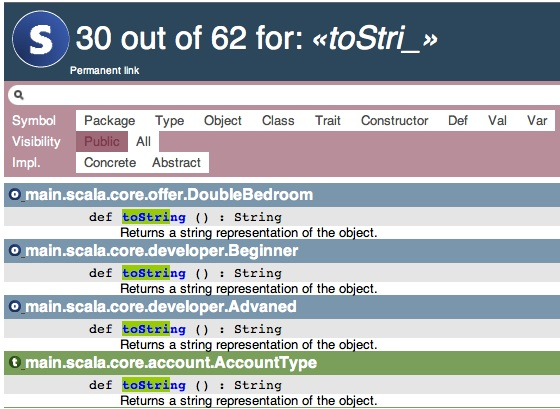
\includegraphics[width=0.7\textwidth]{highlighting}}
\end{center}
\caption{Highlighting Feature}
\label{fig:highlighting}
\end{figure}

\textbf{Infinite Scrolling} (Fig.\ref{fig:infinityscrolling})- allows the user to continuously scroll through search results without having navigate between pages.


\begin{figure}[h!t]
\begin{center}
\leavevmode
\fbox{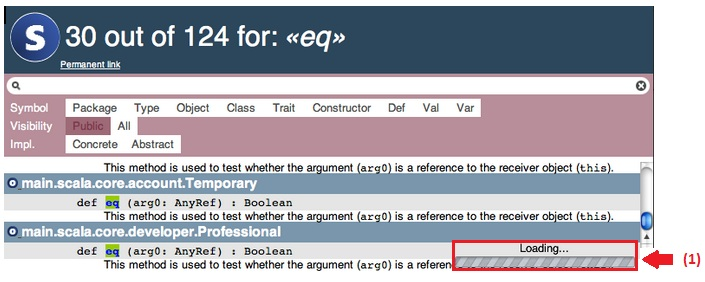
\includegraphics[width=0.7\textwidth]{infinityscrolling}}
\end{center}
\caption{Infinite scrolling feature. The loading image (1) appears to notify the user that more results are being fetched.}
\label{fig:infinityscrolling}
\end{figure}

\textbf{Other nice-to-have features} 
We added some handy shortcuts to help users navigate to the main search box. We integrated google search to help the user search in Google if his query produces no results. 

\subsubsection{Intuitive Query Syntax}
Colladoc Smart Search supports Scala-like search syntax for queries, which makes searching natural for any Scala developer. We allow searching for advanced language constructs such as currying, lambda expressions, generic classes and parameters. Additionally, support for query grouping, boolean operators and wildcards allows users to perform searches using familiar constructs from popular search engines.   
Testing

The Colladoc Smart Search project includes a variety of tests that provide comprehensive test coverage of the new functionality added and of the integration points between this new functionality and the original product.

We have added 211 new tests to Colladoc. Metrics show that our tests achieve 92\% code coverage of the new components that we added (Fig.~\ref{fig:codecoverage}). In addition, our tests achieve 56\% code coverage for the entire Colladoc codebase, which previously had no test coverage.

\begin{figure}[h!t]
\begin{center}
\leavevmode
\subfigure[Colladoc Smart Search Code]{\label{fig:codecoverage-a}
\fbox{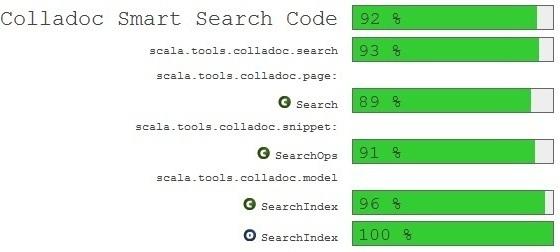
\includegraphics[width=0.4\textwidth]{codecoverage_smartsearch}}}
\subfigure[Colladoc Total]{\label{fig:codecoverage-b}
\fbox{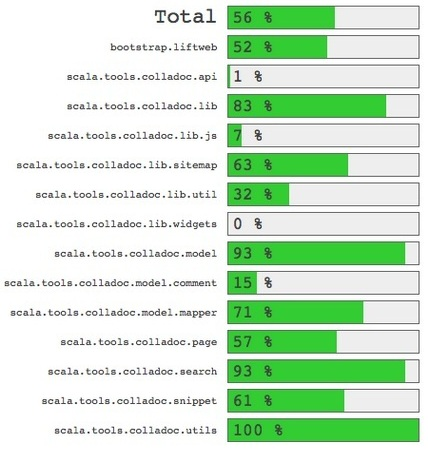
\includegraphics[width=0.4\textwidth]{codecoverage_total}}}
\end{center}
\caption{Code Coverage Results. The results are generated using SCCT}
\label{fig:codecoverage}
\end{figure}

\subsection{Performance}
We thoroughly tested Colladoc performance using several two large code bases-Lift Web Framework and Scala Library. We also use several small projects (see Table \ref{tab:test-projects})

\begin{table}
\begin{tabular}{|p{0.9in}|p{2.2in}|p{1.2in}|} \hline 
Code Base & Entities for indexing & Indexing (ms)\\ \hline 
Scala Library & 85 495\newline ( 572 scala files containing approximately 50 packages, over 1000 classes, objects and traits ) & 190 000 \\ \hline 
Lift-total & 85 902\newline (300 scala files, containing approximately 59 packages, over 1500 classes, objects and traits) &  \\ \hline 
Lift-base & 38 379 & 41709\\ \hline
Lift-modules & 18 747 & 20132\\ \hline
Lift-json &	2232 & 4370\\ \hline
Demo-Project &	1873 & 3863\\ \hline
\end{tabular}
\caption{Test Projects}
\label{tab:test-projects}
\end{table}

\textbf{Indexing performance}\\
Indexing of the documentation model for the Scala Standard Library codebase finishes in approximately 190 seconds on the Imperial College DoC lab machines. Since indexing is done only when the web application is launched, this performance is acceptable.

Fig.~\ref{fig:indexing-performance}  shows the results of indexing performance on documentation models of varying size. These results clearly show that our indexing algorithm scales well with the size of the documentation model being indexed. The linear growth in indexing time is evidence that the complexity of our indexing algorithm is ϴ(n).

\begin{figure}[h!t]
\begin{center}
\leavevmode
\fbox{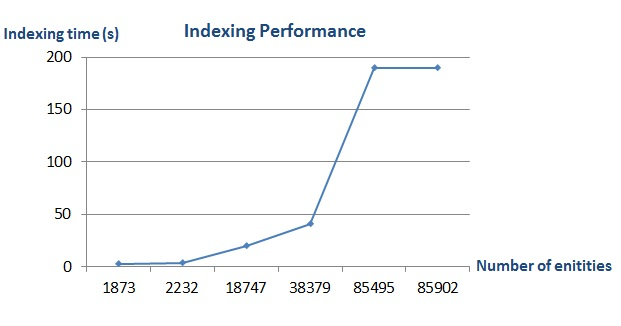
\includegraphics[width=0.9\textwidth]{indexing-performance}}
\end{center}
\caption{Search Performance}
\label{fig:indexing-performance}
\end{figure}

\textbf{Search performance}\\
Search performance on these large source codebases is very good, even for search queries that return up to 80,000 total results. Stop-watch search performance tests using several different machine configurations \emph{\color{red}(give some example machine specs here?)}, show that the first set of search results are presented to the user in less than two seconds on average. Figure \ref{fig:search-performance} depicts programmatic measurements of the time taken execute a query for different numbers of total search results. This graph shows that the time taken to execute a search is not related to total number results since we have logic to only actually fetch indexed documents for the first "page" of results. Furthermore, this highlights the fact that the product provides consistent search throughput regardless of the total number of results for a query.


\begin{figure}[h!t]
\begin{center}
\leavevmode
\fbox{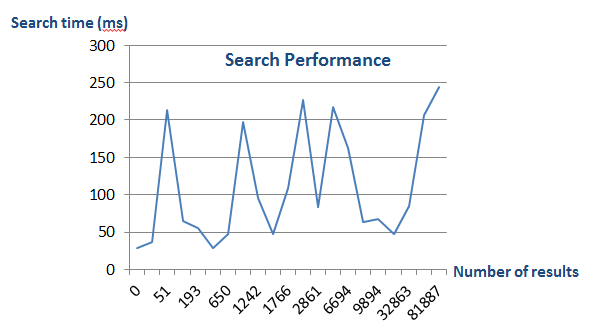
\includegraphics[width=0.9\textwidth]{search-performance}}
\end{center}
\caption{Search Performance}
\label{fig:search-performance}
\end{figure}


Performance testing clearly shows that Colladoc Smart Search provides acceptable performance for our user scenarios. Additionally, the performance of non-Smart Search Colladoc scenarios have not been degraded.